%TODO : expliquer quelque part le paramètre de length estimator (3, 5 ou 8)

\section{Comparison and interpretation of results for the train}

The purpose of this section is to interpret and compare results on different pictures deblurred by the three methods of deconvolution used: Lucy-Richardson, Wiener and regularization. We will test essentially ideal images artificially blurred in order to isolate the influence of certain parameters. Although most of the images used are not taken inside of a train as it indicated, the assumption of a linear motion blur is well respected and we are therefore in the first case treated (the train).

\subsection{Noise influence}

We are interested in deblurring a original image with noise (that is independent of signal). Three different cases are considered: the original image without noise, with Gaussian noise (mean equals $0$ and variance $0.01$) and with (very light) speckle noise. The original image has been artificially blurred and pictures were compressed during treatment (see section [???]). The noise was inserted by predefined functions of Matlab. The results are shown in figure ?????:

\begin{figure}[h]
\centering
\begin{subfigure}{0.32\textwidth}
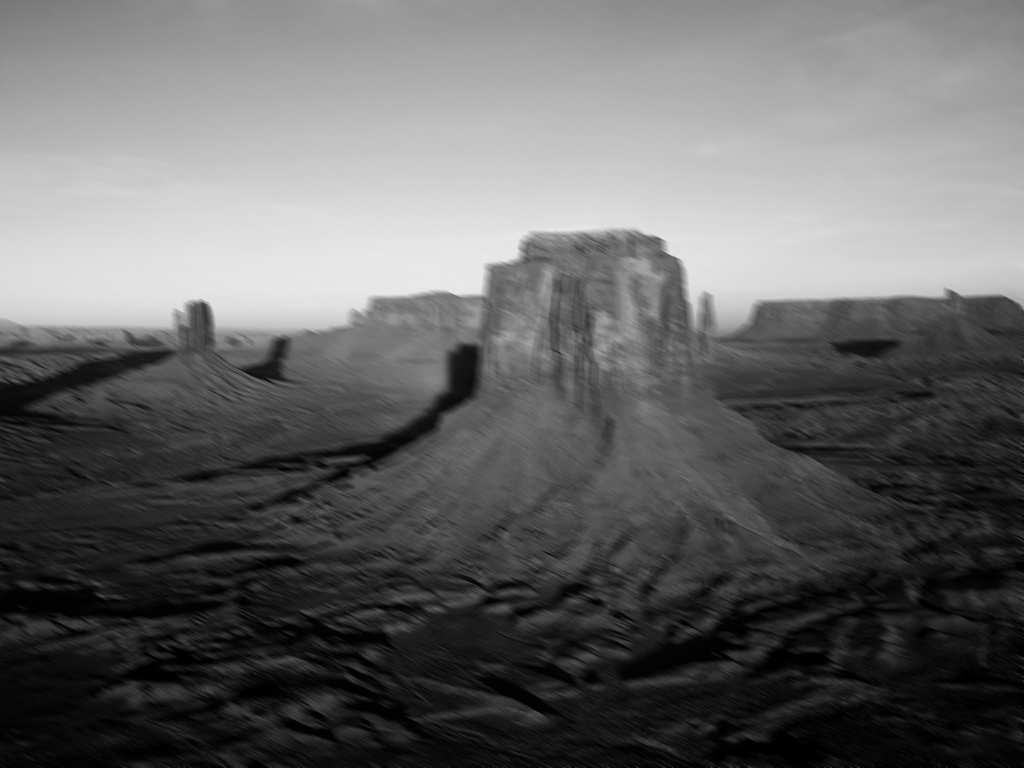
\includegraphics[width= \textwidth]{../Images/Results/desert/Normal/input.png}
\vspace{-30pt}
\caption{Picture deblurred using only a $256\times 256$ centered crop of the picture. }
\label{fig:NormalI}
\end{subfigure}
~
\begin{subfigure}{0.32\textwidth}
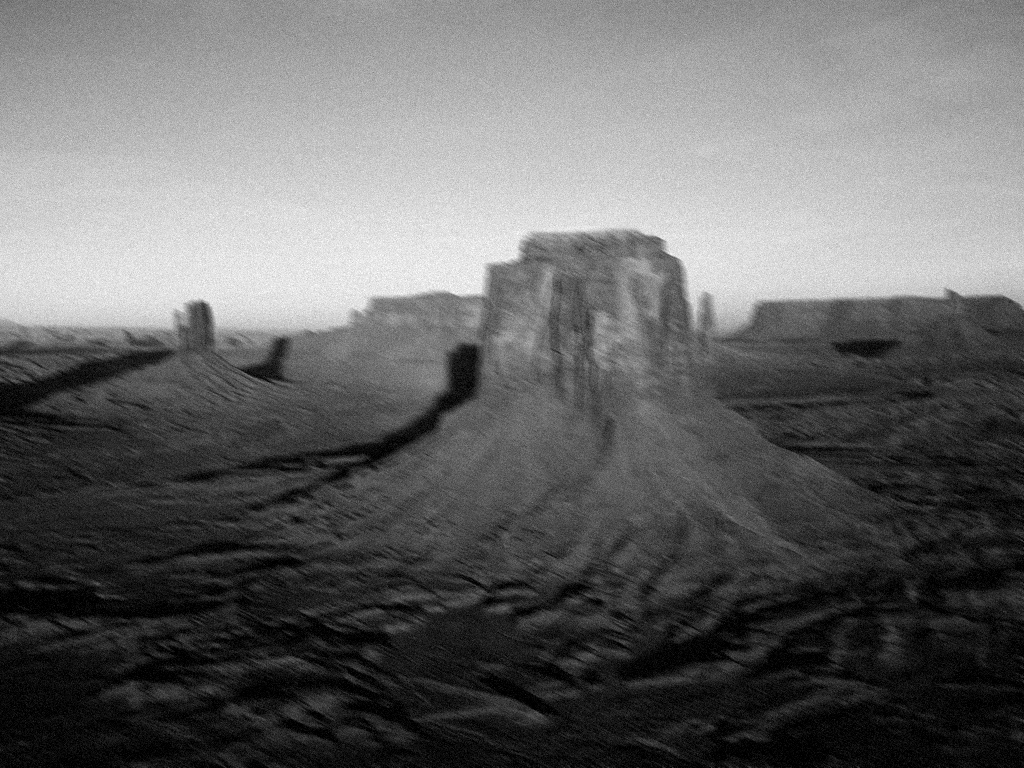
\includegraphics[{width= \textwidth}]{../Images/Results/desert/Gauss/input.png}
\vspace{-30pt}
\caption{Picture deblurred using the whole image.}
\label{fig:GaussI}
\end{subfigure}
~
\begin{subfigure}{0.32\textwidth}
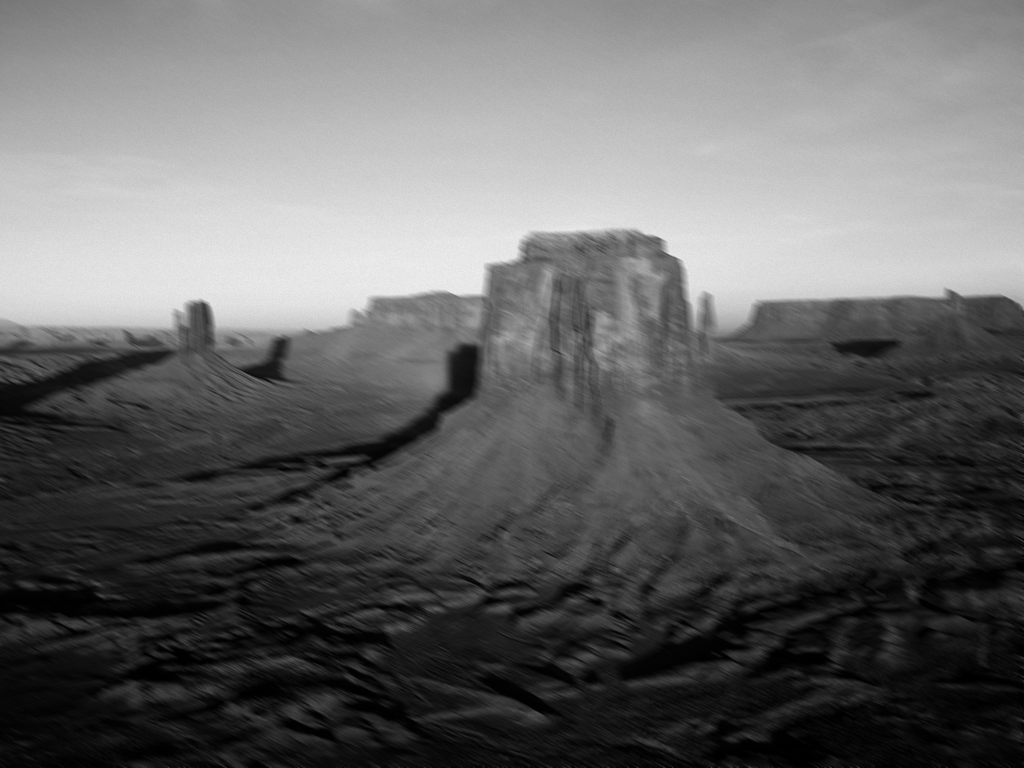
\includegraphics[{width= \textwidth}]{../Images/Results/desert/Speckle/input.png}
\vspace{-30pt}
\caption{Picture deblurred using the whole image.}
\label{fig:SpeckleI}
\end{subfigure}
~
\begin{subfigure}{0.32\textwidth}
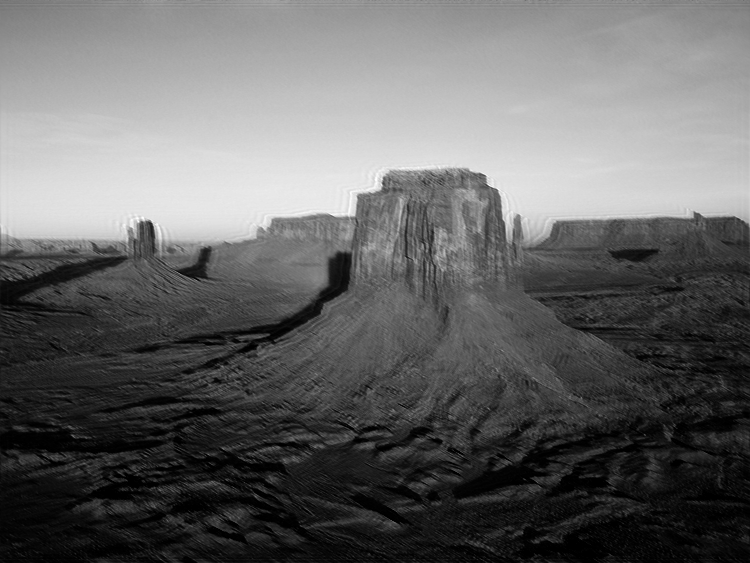
\includegraphics[{width= \textwidth}]{../Images/Results/desert/Normal/L.png}
\vspace{-30pt}
\caption{Picture deblurred using the whole image.}
\label{fig:NormalL}
\end{subfigure}
\caption{Different matrix's size for the PSF estimation.}
\end{figure}

\begin{figure}

\begin{subfigure}{0.32\textwidth}
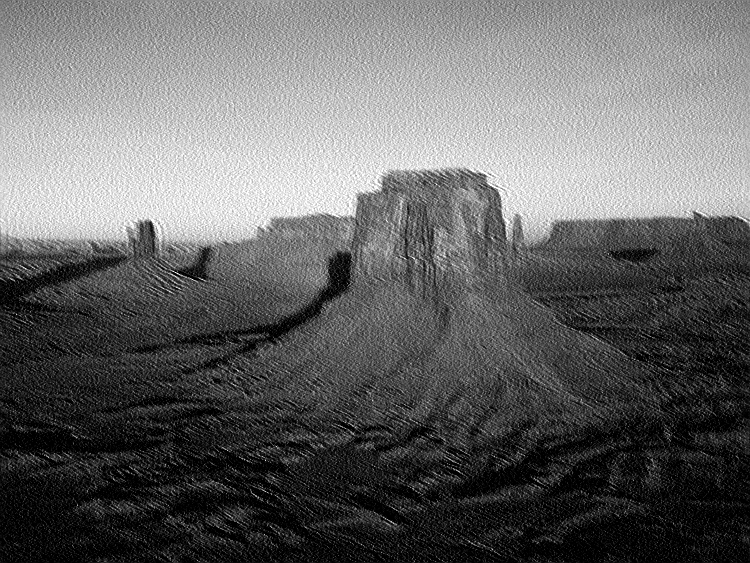
\includegraphics[{width= \textwidth}]{../Images/Results/desert/Gauss/L.png}
\vspace{-30pt}
\caption{Picture deblurred using the whole image.}
\label{fig:GaussL}
\end{subfigure}
~
\begin{subfigure}{0.32\textwidth}
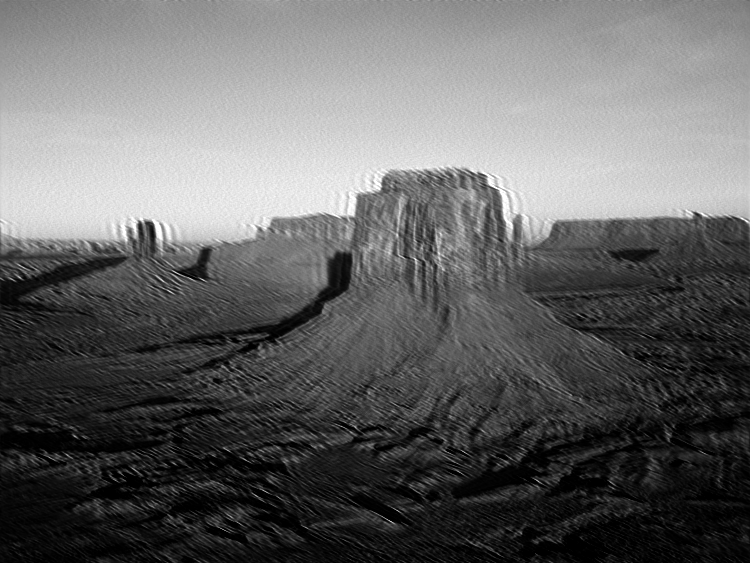
\includegraphics[{width= \textwidth}]{../Images/Results/desert/Speckle/L.png}
\vspace{-30pt}
\caption{Picture deblurred using the whole image.}
\label{fig:SpeckleL}
\end{subfigure}
~
\begin{subfigure}{0.32\textwidth}
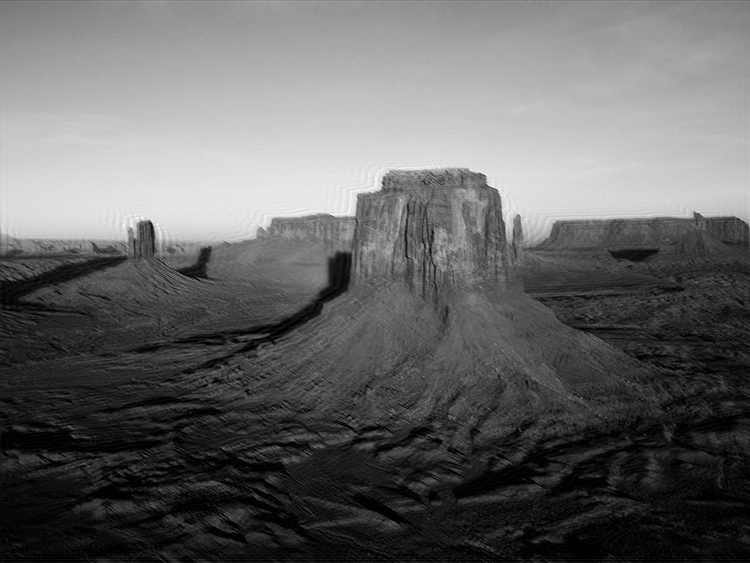
\includegraphics[{width= \textwidth}]{../Images/Results/desert/Normal/W.png}
\vspace{-30pt}
\caption{Picture deblurred using the whole image.}
\label{fig:NormalW}
\end{subfigure}
~
\begin{subfigure}{0.32\textwidth}
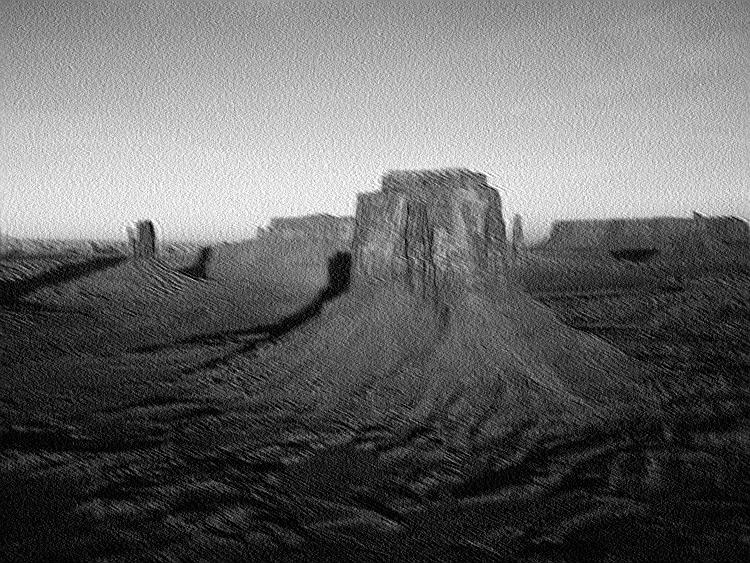
\includegraphics[{width= \textwidth}]{../Images/Results/desert/Gauss/W.png}
\vspace{-30pt}
\caption{Picture deblurred using the whole image.}
\label{fig:GaussW}
\end{subfigure}
~
\begin{subfigure}{0.32\textwidth}
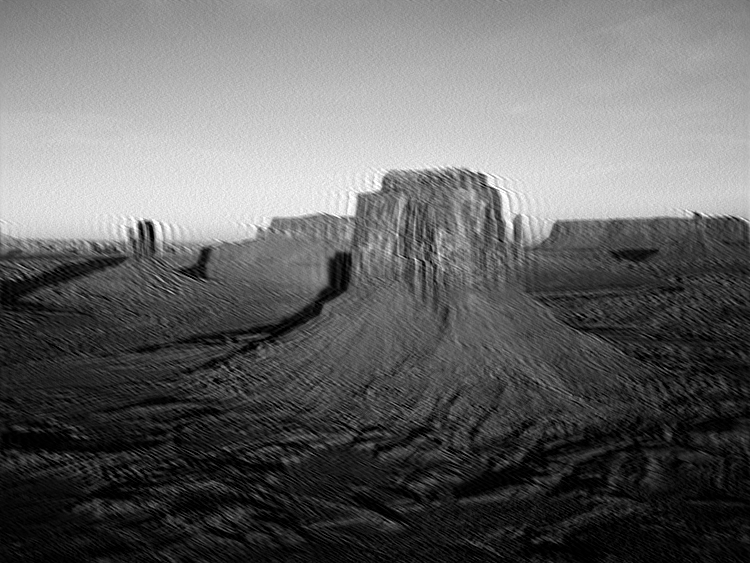
\includegraphics[{width= \textwidth}]{../Images/Results/desert/Speckle/W.png}
\vspace{-30pt}
\caption{Picture deblurred using the whole image.}
\label{fig:SpeckleW}
\end{subfigure}
~
\begin{subfigure}{0.32\textwidth}
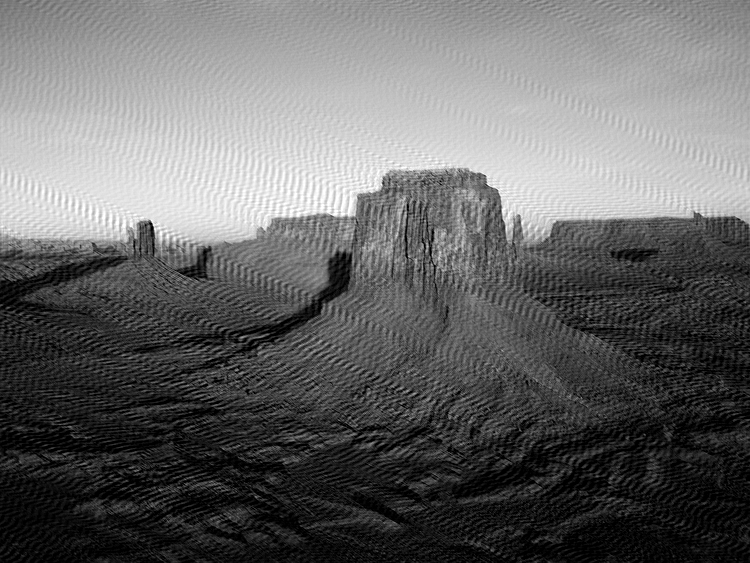
\includegraphics[{width= \textwidth}]{../Images/Results/desert/Normal/R.png}
\vspace{-30pt}
\caption{Picture deblurred using the whole image.}
\label{fig:NormalR}
\end{subfigure}
~
\begin{subfigure}{0.32\textwidth}
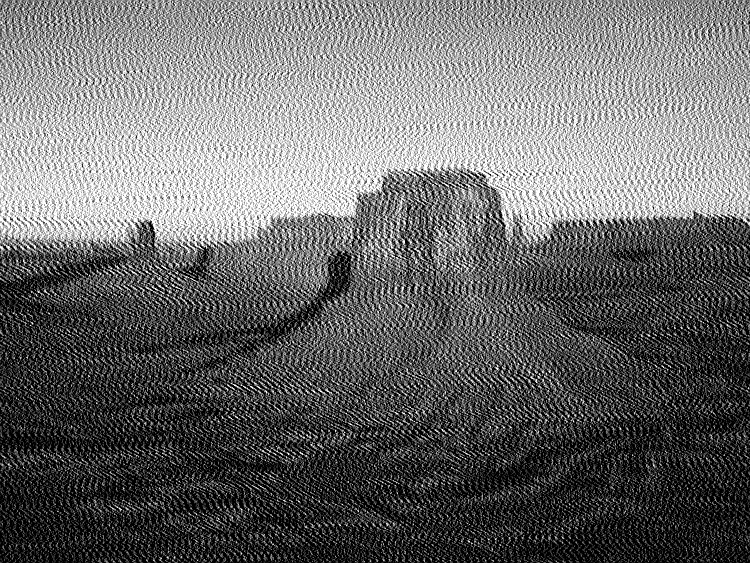
\includegraphics[{width= \textwidth}]{../Images/Results/desert/Gauss/R.png}
\vspace{-30pt}
\caption{Picture deblurred using the whole image.}
\label{fig:GaussR}
\end{subfigure}
~
\begin{subfigure}{0.32\textwidth}
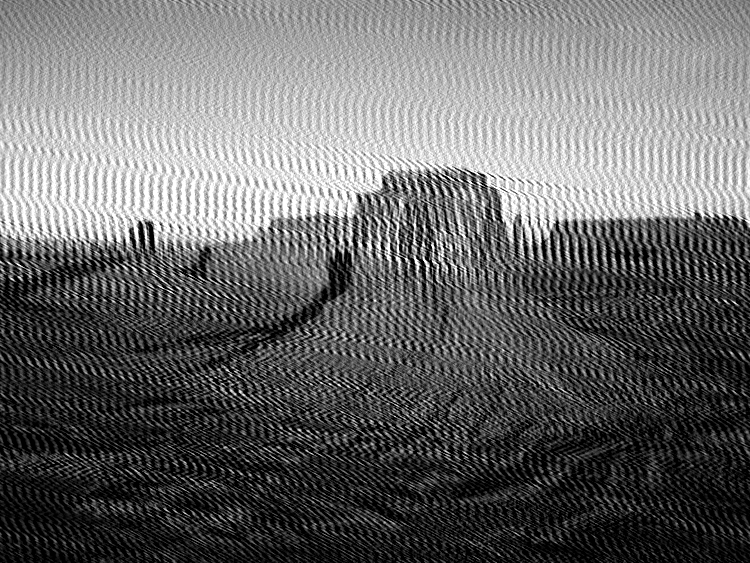
\includegraphics[{width= \textwidth}]{../Images/Results/desert/Speckle/R.png}
\vspace{-30pt}
\caption{Picture deblurred using the whole image.}
\label{fig:SpeckleR}
\end{subfigure}
\caption{Different matrix's size for the PSF estimation.}
\end{figure}


We note that the algorithm reguralisation is much more sensitive to the presence of noise in the original image, for both type of noise injected at the start. The other two methods are also affected but the deblurring is not compromised (provided that the initial noise is not too important).

%TODO : possible d'expliquer ça mathématiquement ? 

\subsection{Length estimator parameter}

To estimate the PSF, it is necessary to estimate the length parameter of blurring (see section [ ??? ]). It's interesting to study the impact of this factor on the output and establish the sensitivity of the three methods used.
The image used here is the famous photo taken in 1972 of Lena, playmate of playboy magazine, and is often used as test algorithms for image processing( REFERENCE TO WIKIPEDIA ). It has been artificially blurred here by an angle of 20 degrees and a length of 30 pixels. The principle is to fix the estimated length for the deblurring in order to see the influence of this value to the final result (it should be noted that the angle estimatated by this algorithm is 20 degrees what is right and so the length parameter is the only variable here). For each method, three cases were treated: the estimated length (that is fixed) is 20 pixels, 30 pixels (exact value) and 40 pixels.  The results are shown in figure ?????:

\begin{figure}[h]
\centering
\begin{subfigure}{0.4\textwidth}
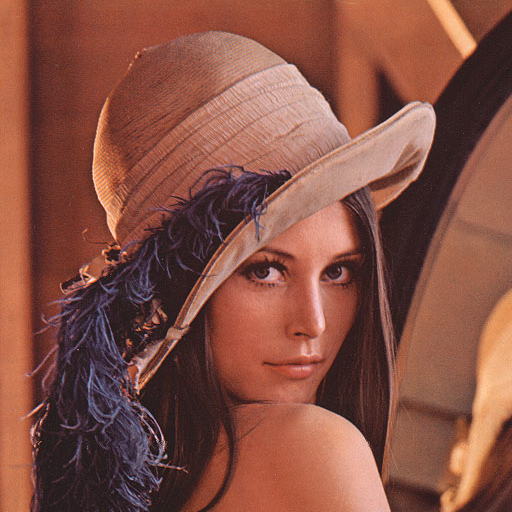
\includegraphics[width= \textwidth]{../Images/Results/Lena/Blur20deg30length/lenaOriginal.png}
\vspace{-30pt}
\caption{Picture deblurred using only a $256\times 256$ centered crop of the picture. }
\label{fig:LOriginal}
\end{subfigure}
~
\begin{subfigure}{0.4\textwidth}
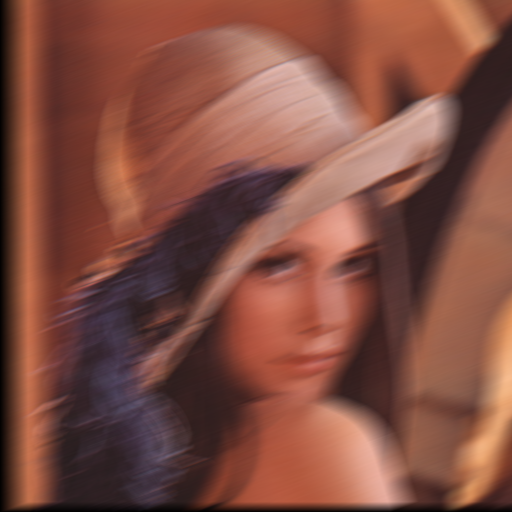
\includegraphics[{width= \textwidth}]{../Images/Results/Lena/Blur20deg30length/ArtificialBlurred.png}
\vspace{-30pt}
\caption{Picture deblurred using the whole image.}
\label{fig:LenaBlurred}
\end{subfigure}
\end{figure}

\begin{figure}[h]
\centering
\begin{subfigure}{0.32\textwidth}
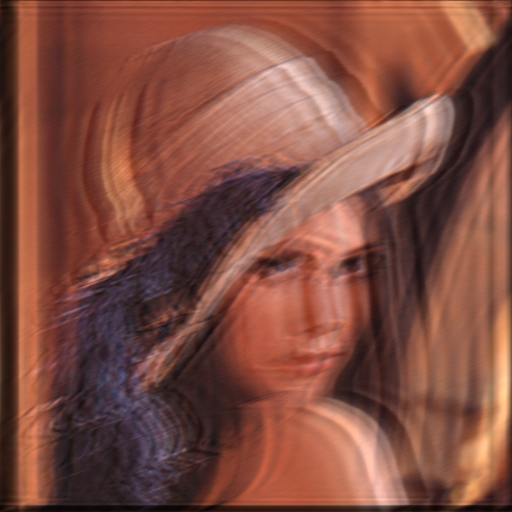
\includegraphics[width= \textwidth]{../Images/Results/Lena/Blur20deg30length/L20.png}
\vspace{-30pt}
\caption{Picture deblurred using only a $256\times 256$ centered crop of the picture. }
\label{fig:L20}
\end{subfigure}
\caption{Different matrix's size for the PSF estimation.}
~
\begin{subfigure}{0.32\textwidth}
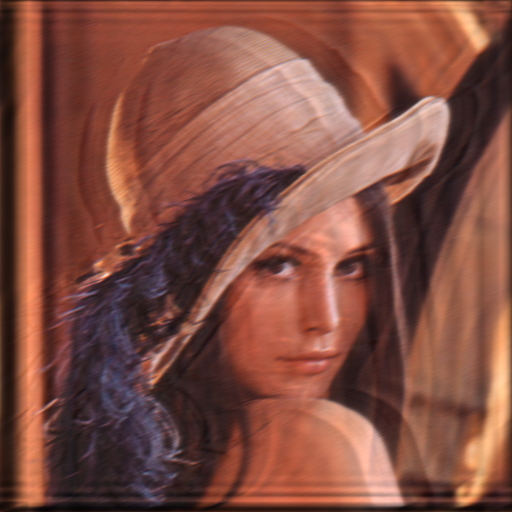
\includegraphics[{width= \textwidth}]{../Images/Results/Lena/Blur20deg30length/L30.png}
\vspace{-30pt}
\caption{Picture deblurred using the whole image.}
\label{fig:L30}
\end{subfigure}
~
\begin{subfigure}{0.32\textwidth}
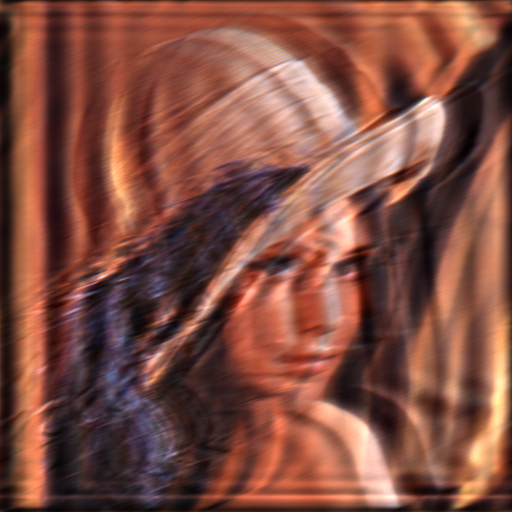
\includegraphics[{width= \textwidth}]{../Images/Results/Lena/Blur20deg30length/L40.png}
\vspace{-30pt}
\caption{Picture deblurred using the whole image.}
\label{fig:L40}
\end{subfigure}
\caption{Different matrix's size for the PSF estimation.}
\end{figure}

\begin{figure}
\begin{subfigure}{0.32\textwidth}
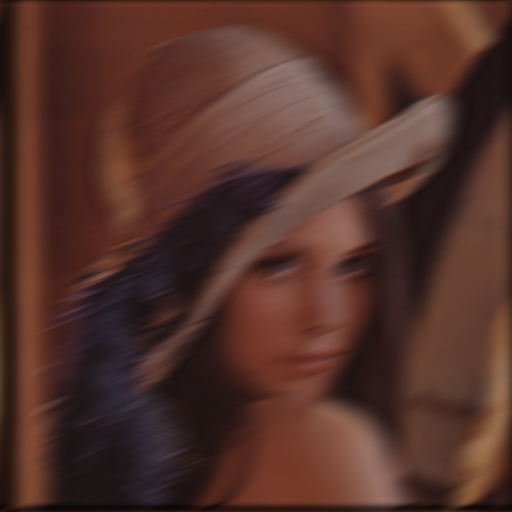
\includegraphics[{width= \textwidth}]{../Images/Results/Lena/Blur20deg30length/W20.png}
\vspace{-30pt}
\caption{Picture deblurred using the whole image.}
\label{fig:W20}
\end{subfigure}
~
\begin{subfigure}{0.32\textwidth}
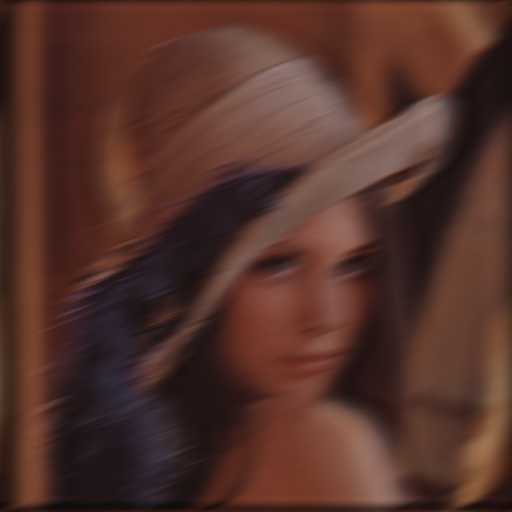
\includegraphics[{width= \textwidth}]{../Images/Results/Lena/Blur20deg30length/W30.png}
\vspace{-30pt}
\caption{Picture deblurred using the whole image.}
\label{fig:W30}
\end{subfigure}
~
\begin{subfigure}{0.32\textwidth}
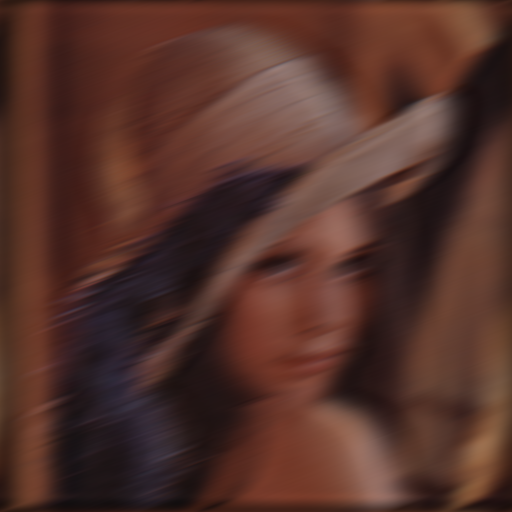
\includegraphics[{width= \textwidth}]{../Images/Results/Lena/Blur20deg30length/W40.png}
\vspace{-30pt}
\caption{Picture deblurred using the whole image.}
\label{fig:W40}
\end{subfigure}
~
\begin{subfigure}{0.32\textwidth}
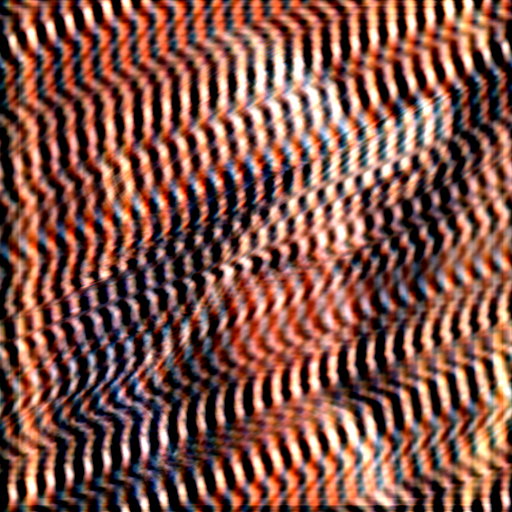
\includegraphics[{width= \textwidth}]{../Images/Results/Lena/Blur20deg30length/R20.png}
\vspace{-30pt}
\caption{Picture deblurred using the whole image.}
\label{fig:R20}
\end{subfigure}
~
\begin{subfigure}{0.32\textwidth}
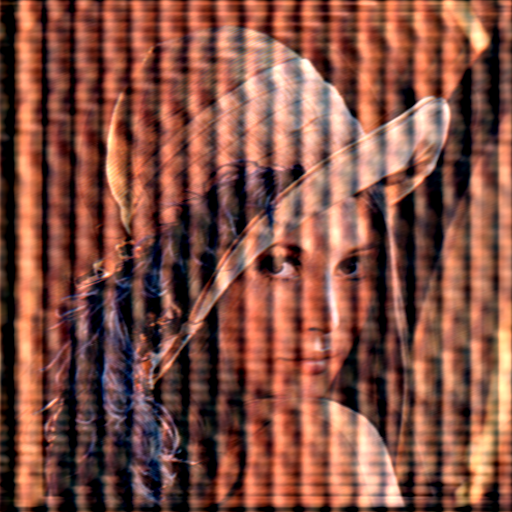
\includegraphics[{width= \textwidth}]{../Images/Results/Lena/Blur20deg30length/R30.png}
\vspace{-30pt}
\caption{Picture deblurred using the whole image.}
\label{fig:R30}
\end{subfigure}
\caption{Different matrix's size for the PSF estimation.}
\end{figure}

\begin{figure}
\begin{subfigure}{0.32\textwidth}
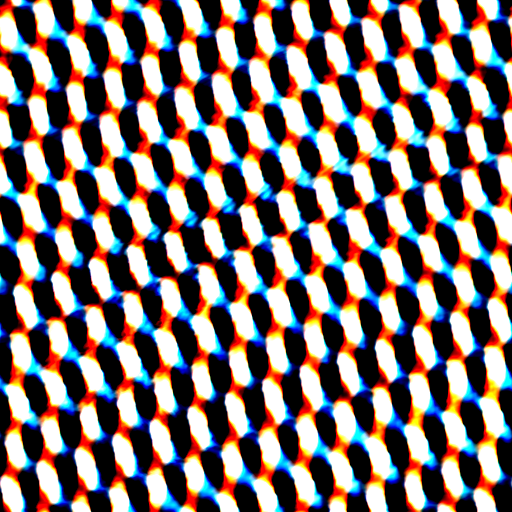
\includegraphics[{width= \textwidth}]{../Images/Results/Lena/Blur20deg30length/R40.png}
\vspace{-30pt}
\caption{Picture deblurred using the whole image.}
\label{fig:R40}
\end{subfigure}
\end{figure}

It directly seems that the regularization method is much more sensitive to the parameter studied than the two others methods. Indeed, artifacts occur when the estimated parameter departs from the true value. The following example shows it (artificially blurred license plate at 0 degrees and 40 pixels):

\begin{figure}[h]
\centering
\begin{subfigure}{0.4\textwidth}

\includegraphics[{width= \textwidth}]{../Images/Results/plaque/Blur0angle40length/originalimage.jpg}
\vspace{-30pt}
\caption{Picture deblurred using the whole image.}
\label{fig:plaqueO}
\end{subfigure}
~
\begin{subfigure}{0.4\textwidth}

\includegraphics[{width= \textwidth}]{../Images/Results/plaque/Blur0angle40length/ArtificialBlur.png}
\vspace{-30pt}
\caption{Picture deblurred using the whole image.}
\label{fig:plaqueBlur}
\end{subfigure}
\caption{Different matrix's size for the PSF estimation.}
\end{figure}


It directly seems that the regularization method is much more sensitive to the parameter studied than the two others methods. Indeed, artifacts occur when the estimated parameter departs from the true value. The following example shows it (artificially blurred license plate at 0 degrees and 40 pixels):

\begin{figure}
\begin{subfigure}{0.32\textwidth}
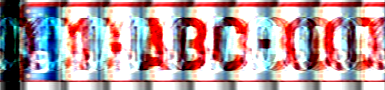
\includegraphics[{width= \textwidth}]{../Images/Results/plaque/Blur0angle40length/RegL38.png}
\vspace{-30pt}
\caption{Picture deblurred using the whole image.}
\label{fig:RegL38}
\end{subfigure}
~
\begin{subfigure}{0.32\textwidth}
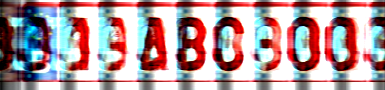
\includegraphics[{width= \textwidth}]{../Images/Results/plaque/Blur0angle40length/RegL39.png}
\vspace{-30pt}
\caption{Picture deblurred using the whole image.}
\label{fig:RegL39}
\end{subfigure}
~
\begin{subfigure}{0.32\textwidth}
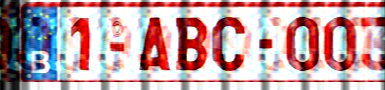
\includegraphics[{width= \textwidth}]{../Images/Results/plaque/Blur0angle40length/RegL40.png}
\vspace{-30pt}
\caption{Picture deblurred using the whole image.}
\label{fig:RegL40}
\end{subfigure}
~
\begin{subfigure}{0.4\textwidth}
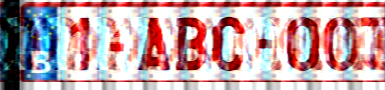
\includegraphics[{width= \textwidth}]{../Images/Results/Lena/Blur20deg30length/RegL41.png}
\vspace{-30pt}
\caption{Picture deblurred using the whole image.}
\label{fig:RegL41}
\end{subfigure}
~
\begin{subfigure}{0.4\textwidth}
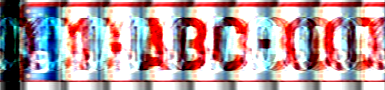
\includegraphics[{width= \textwidth}]{../Images/Results/Lena/Blur20deg30length/RegL42.png}
\vspace{-30pt}
\caption{Picture deblurred using the whole image.}
\label{fig:RegL42}
\end{subfigure}
\caption{Different matrix's size for the PSF estimation.}
\end{figure}


%TODO Y a moyen d'expliquer pourquoi reg est plus sensible mathématiquement vous pensez ? 

\subsection{Compression and computation time}


Our bonus item relates to the time computation of deblurring. It's important to analyze whether the time saved is significant and if it's not compromising quality of deblurred images. For that, we will compare the execution time by compressing or not the original image for the three algorithms. The testing picture is the photo of Lena, artificially blurred to 50 degrees and with a length of 80 pixels.

\begin{figure}[h]
\centering
\begin{subfigure}{0.4\textwidth}
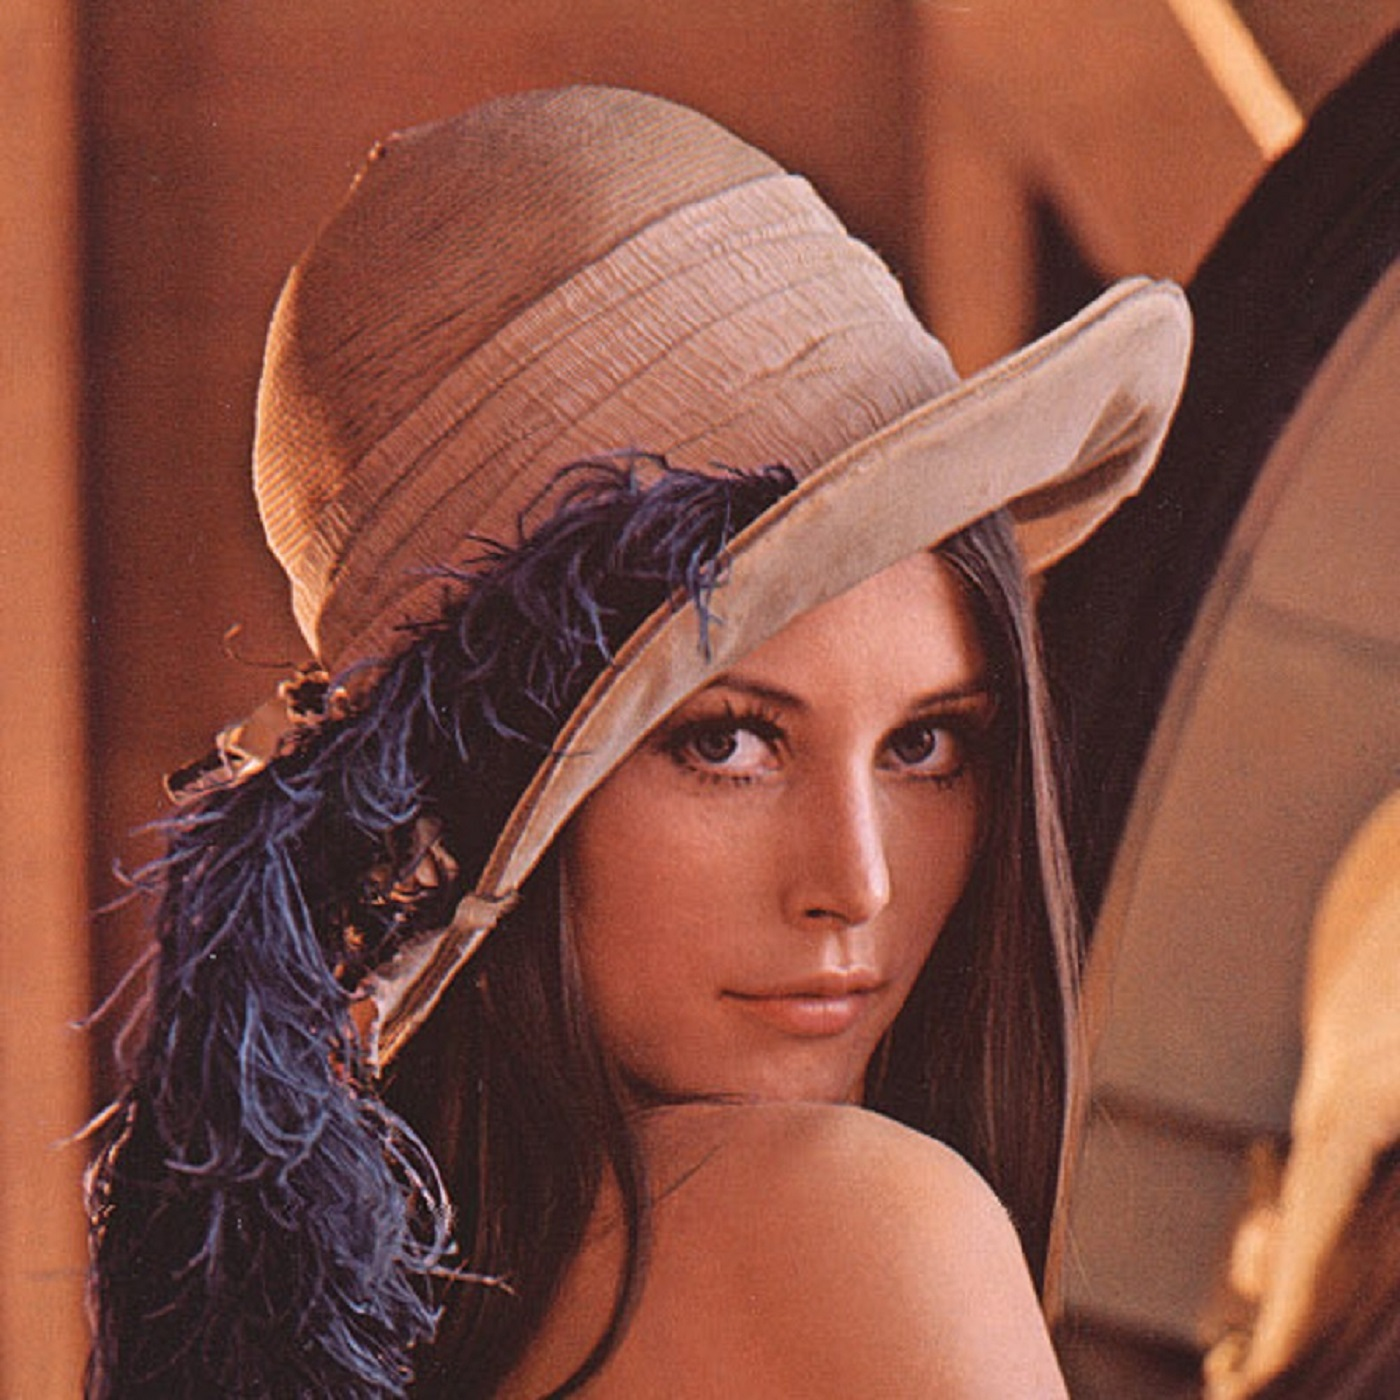
\includegraphics[{width= \textwidth}]{../Images/Results/Lena/Lena2/lena.jpg}
\vspace{-30pt}
\caption{Picture deblurred using the whole image.}
\label{fig:LenaO}
\end{subfigure}
\caption{Different matrix's size for the PSF estimation.}
~
\begin{subfigure}{0.4\textwidth}
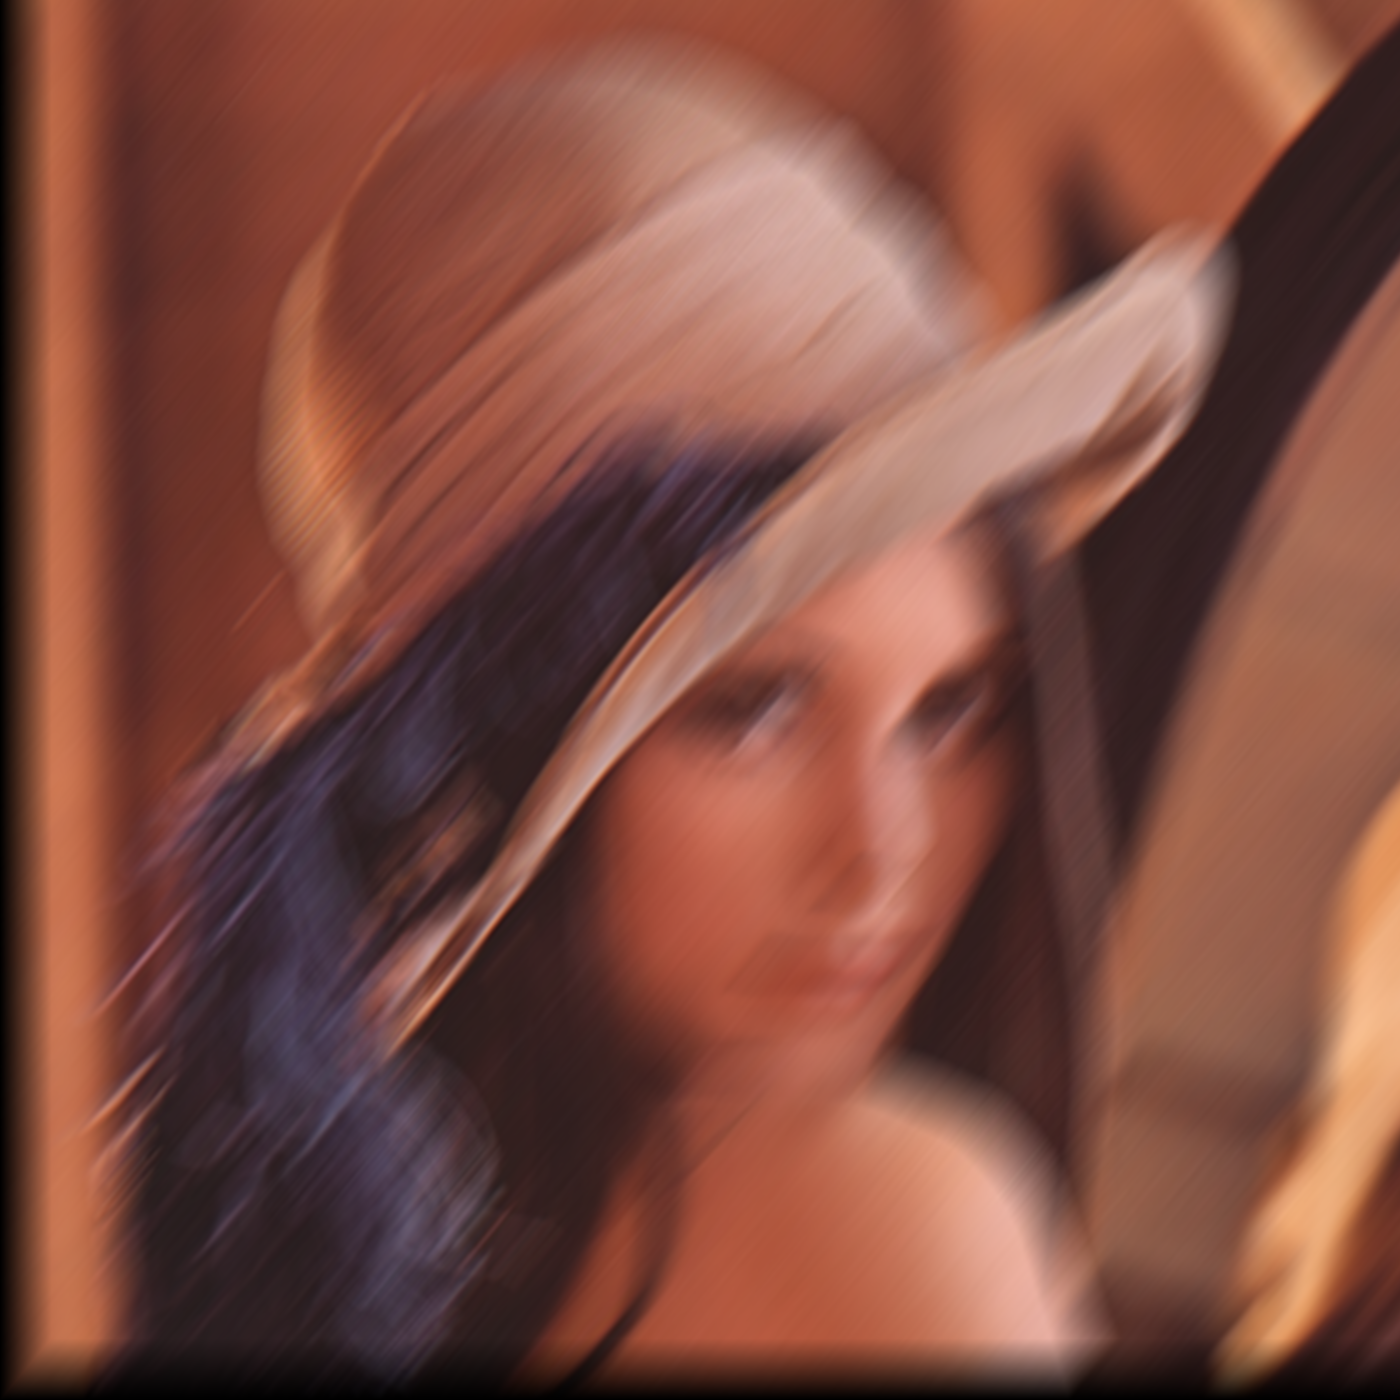
\includegraphics[{width= \textwidth}]{../Images/Results/Lena/Lena2/Blur80a50.png}
\vspace{-30pt}
\caption{Picture deblurred using the whole image.}
\label{fig:Blur80a50}
\end{subfigure}
\caption{Different matrix's size for the PSF estimation.}
\end{figure}

The following table shows the different computation time:

\begin{tabular}{|l|c|c|r|}
  \hline
  & Lucy &  Wiener & regularization \\
  \hline
  Time with compression [s] & 7.4 & 1.15 & 3.3 \\
  \hline
  Time without compression [s]  & 24.2 & 3.36 & 10.13 \\
  \hline
\end{tabular}

\begin{figure}[h]
\centering
\begin{subfigure}{0.32\textwidth}
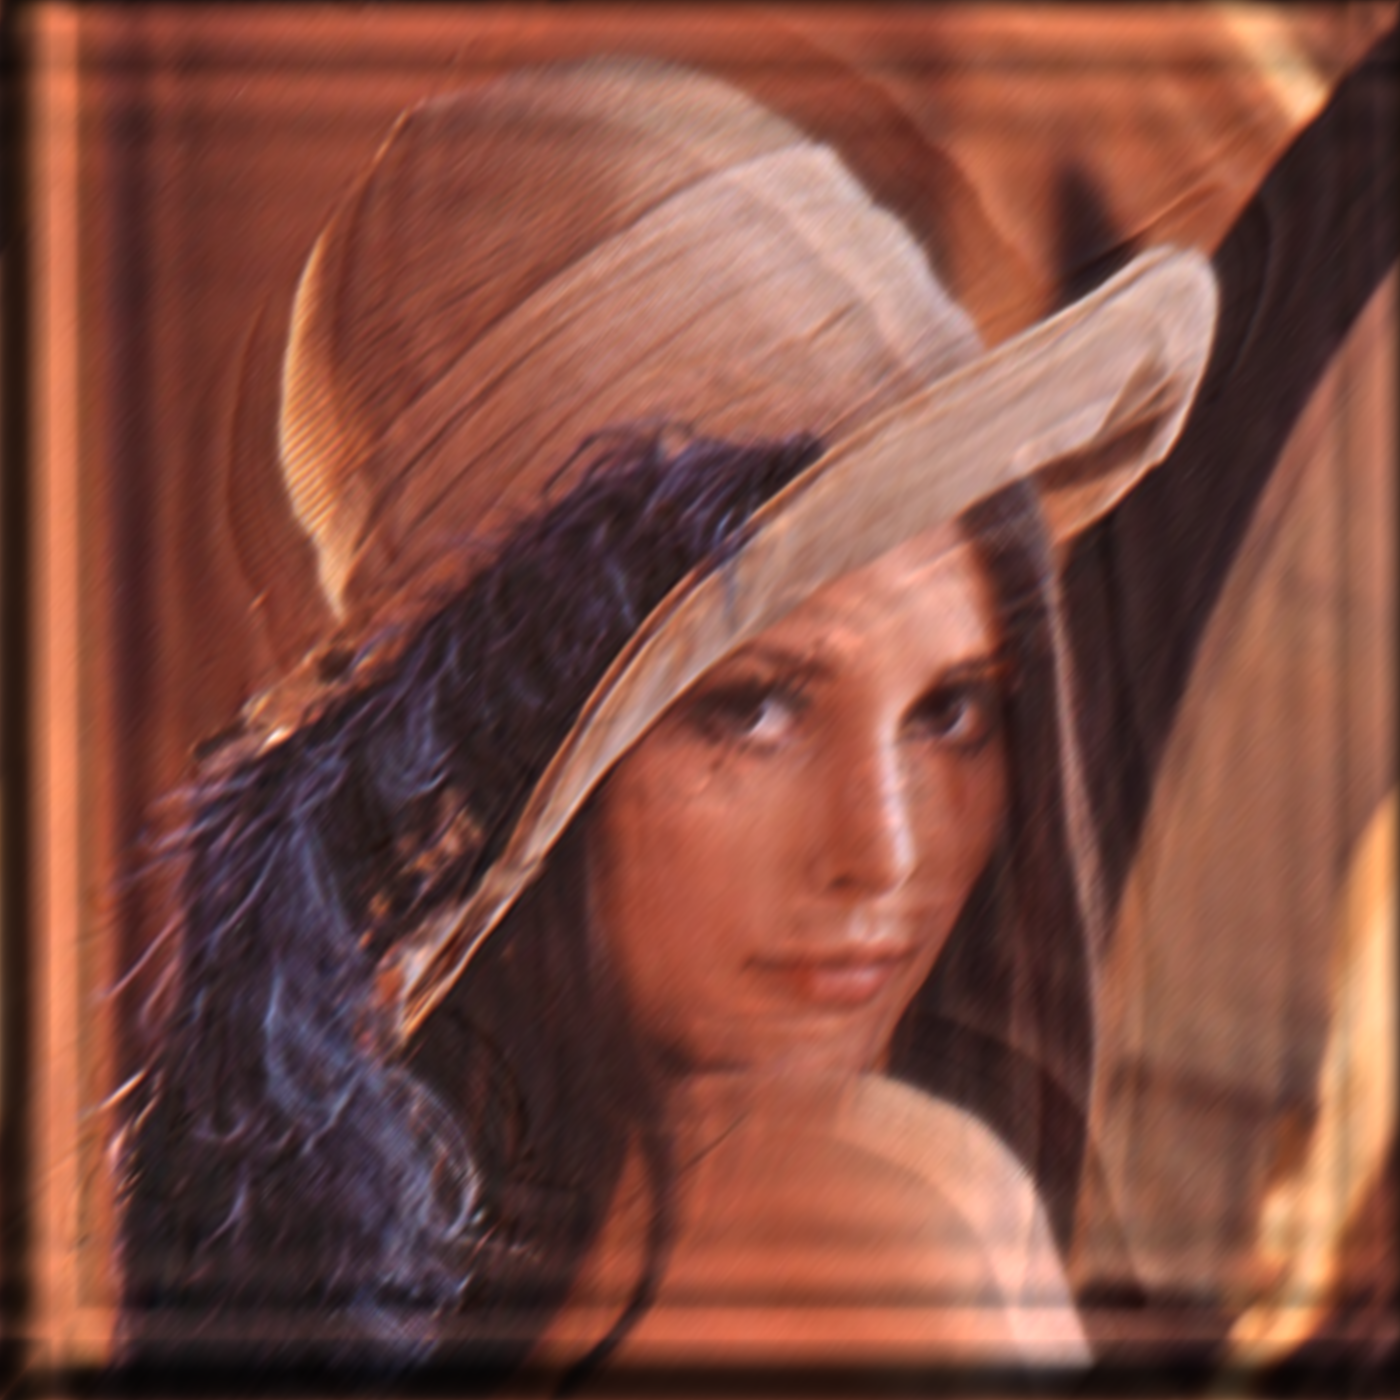
\includegraphics[{width= \textwidth}]{../Images/Results/Lena/Lena2/Lucy.png}
\vspace{-30pt}
\caption{Picture deblurred using the whole image.}
\label{fig:Lulu}
\end{subfigure}
\caption{Different matrix's size for the PSF estimation.}
~
\begin{subfigure}{0.32\textwidth}
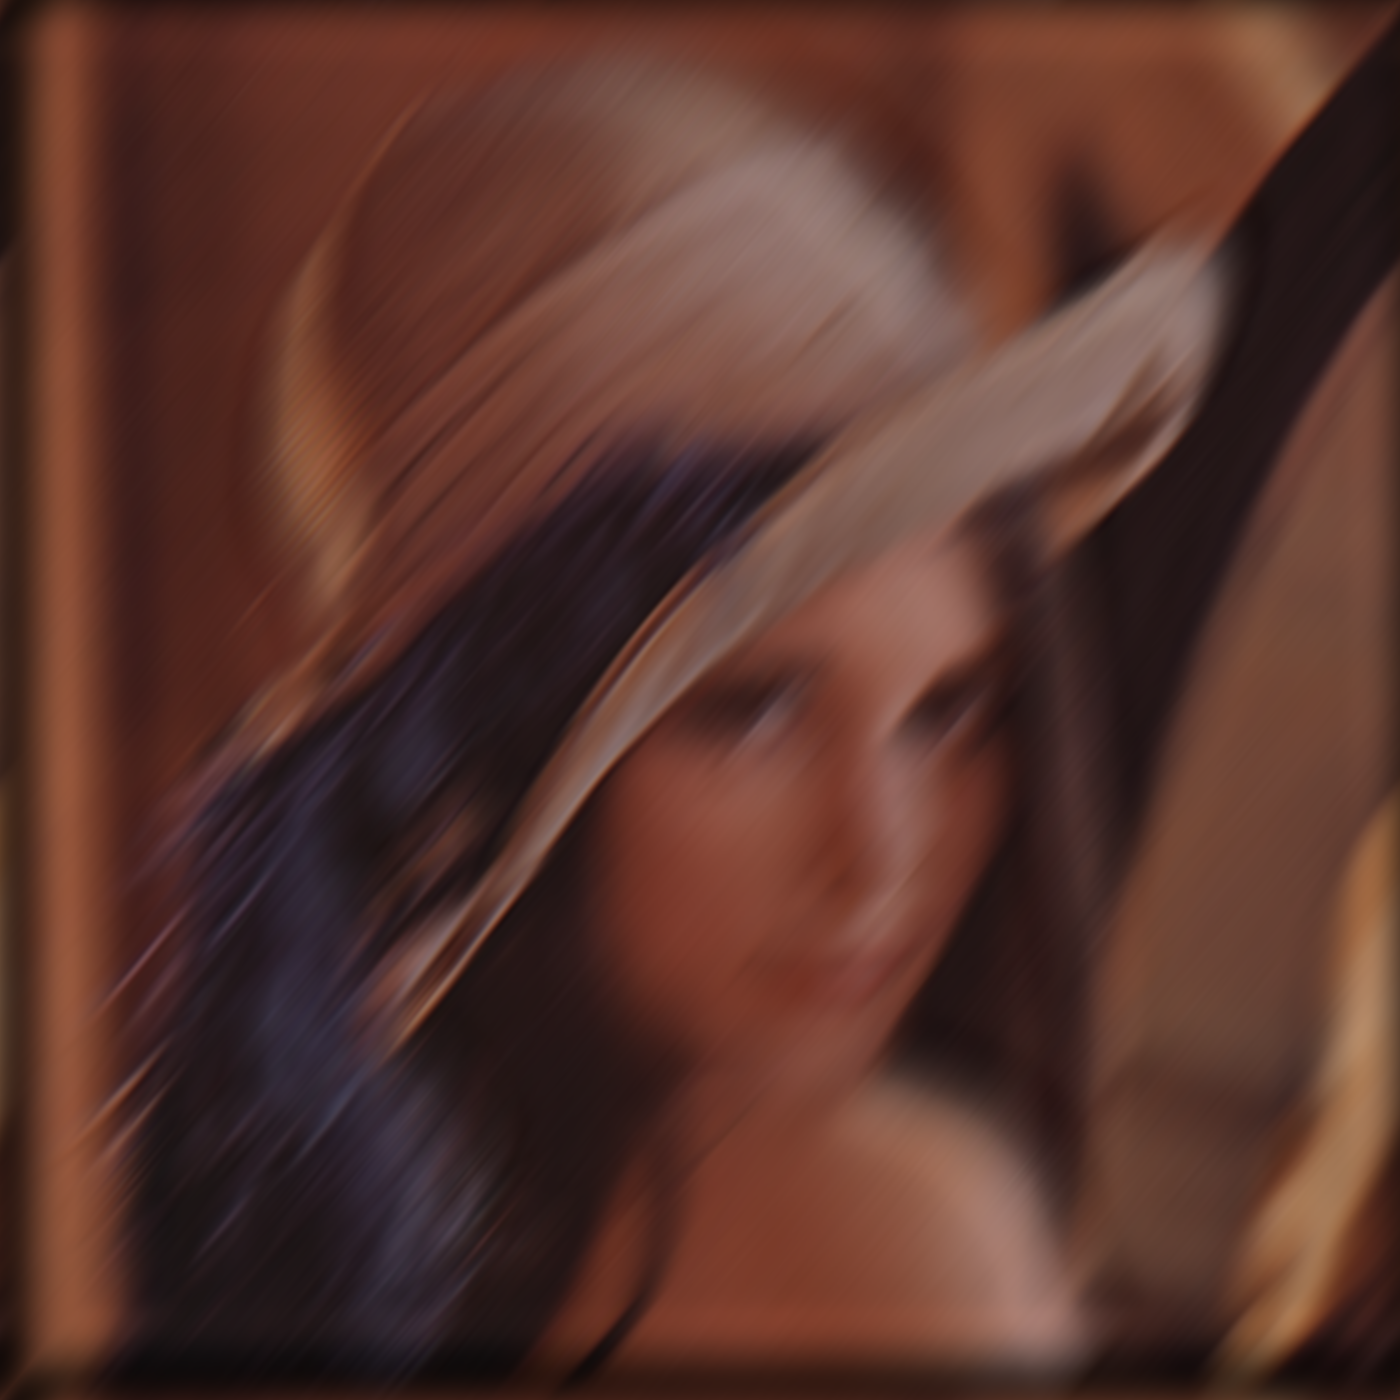
\includegraphics[{width= \textwidth}]{../Images/Results/Lena/Lena2/Wiener.png}
\vspace{-30pt}
\caption{Picture deblurred using the whole image.}
\label{fig:Wiwi}
\end{subfigure}
\caption{Different matrix's size for the PSF estimation.}
~
\begin{subfigure}{0.32\textwidth}
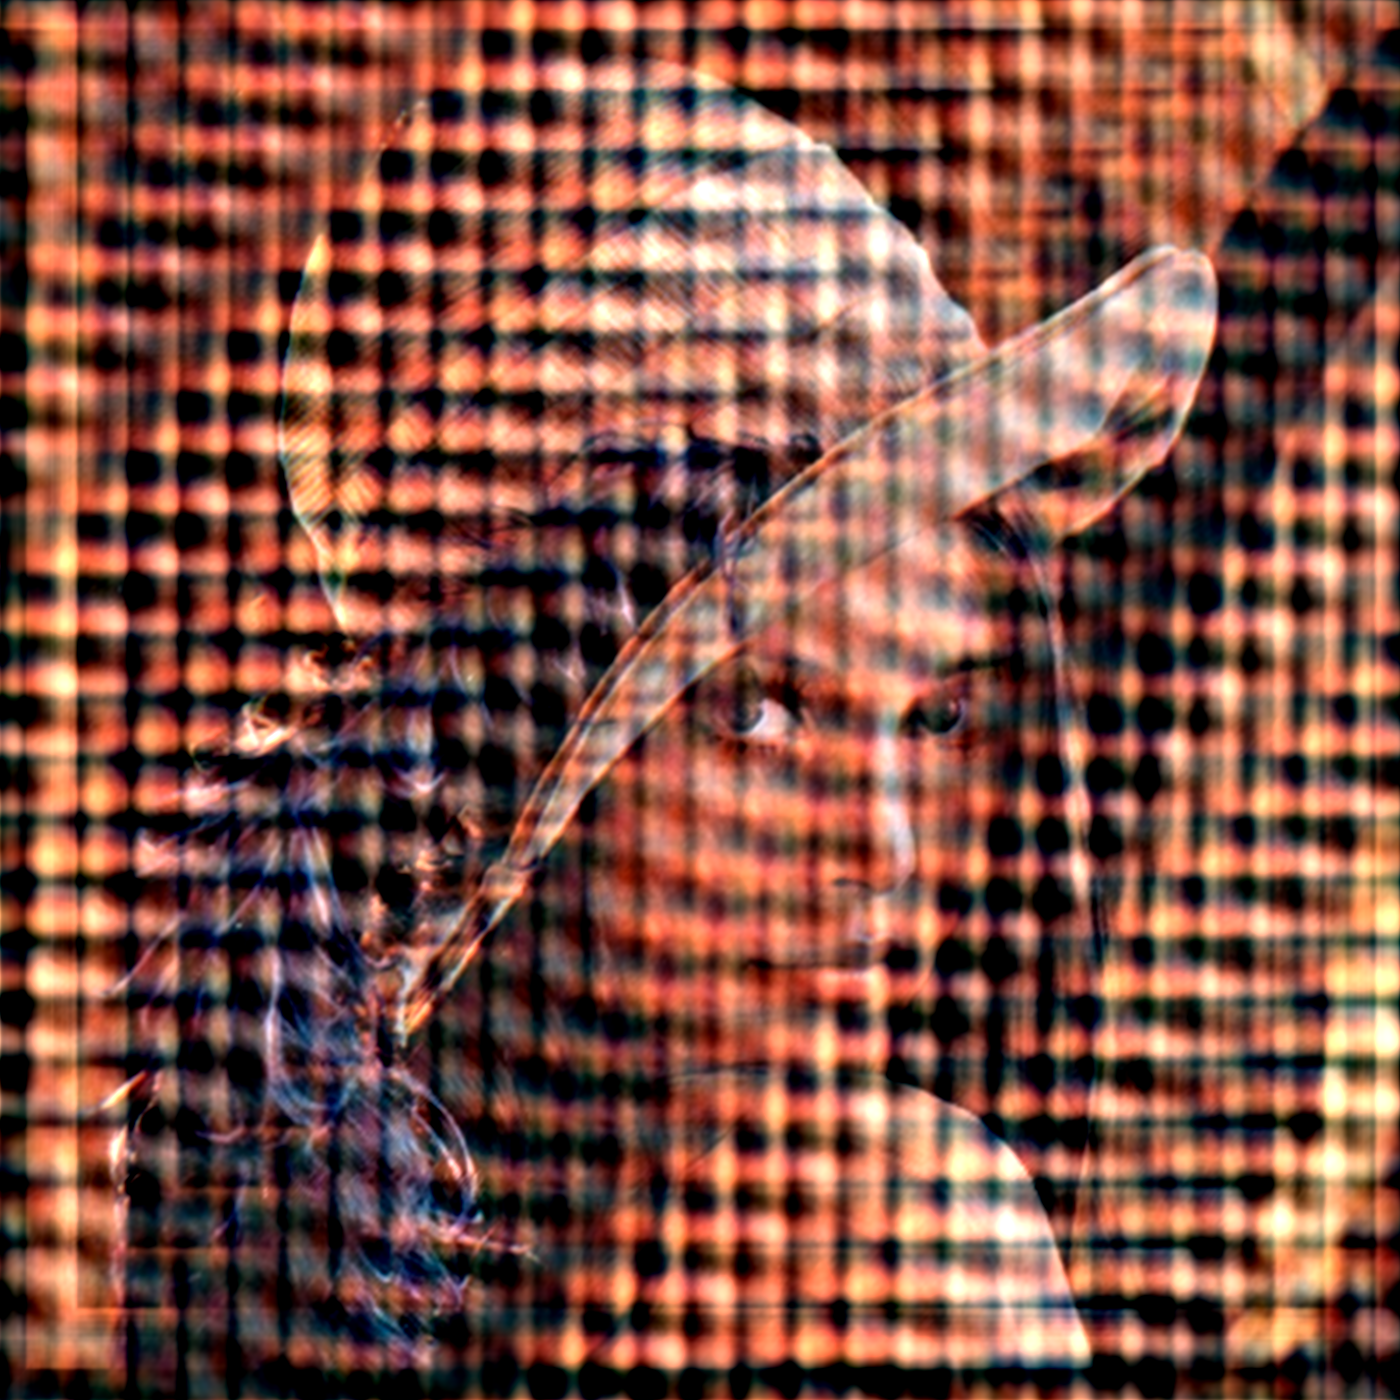
\includegraphics[{width= \textwidth}]{../Images/Results/Lena/Lena2/Reg.png}
\vspace{-30pt}
\caption{Picture deblurred using the whole image.}
\label{fig:Rere}
\end{subfigure}
\caption{Different matrix's size for the PSF estimation.}
~
\begin{subfigure}{0.32\textwidth}
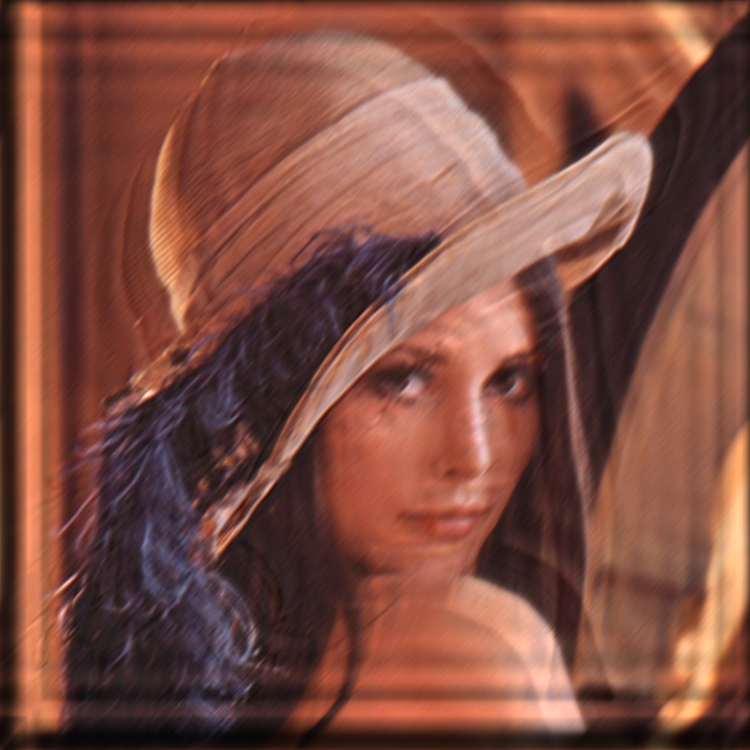
\includegraphics[{width= \textwidth}]{../Images/Results/Lena/Lena2/Lucy-Comp.png}
\vspace{-30pt}
\caption{Picture deblurred using the whole image.}
\label{fig:Lucycomp}
\end{subfigure}
\caption{Different matrix's size for the PSF estimation.}
~
\begin{subfigure}{0.32\textwidth}
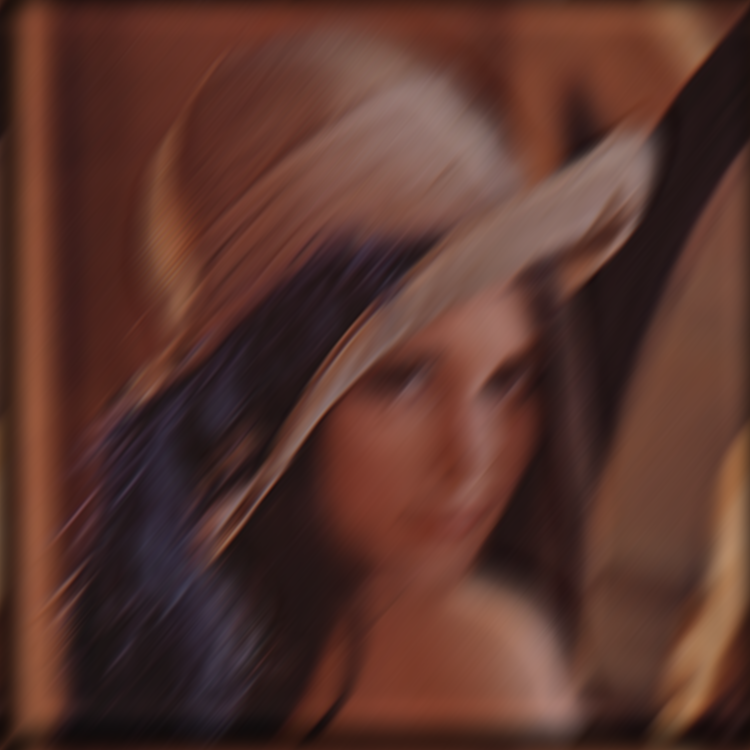
\includegraphics[{width= \textwidth}]{../Images/Results/Lena/Lena2/Wiener-Comp.png}
\vspace{-30pt}
\caption{Picture deblurred using the whole image.}
\label{fig:Wienercomp}
\end{subfigure}
\caption{Different matrix's size for the PSF estimation.}
~
\begin{subfigure}{0.32\textwidth}
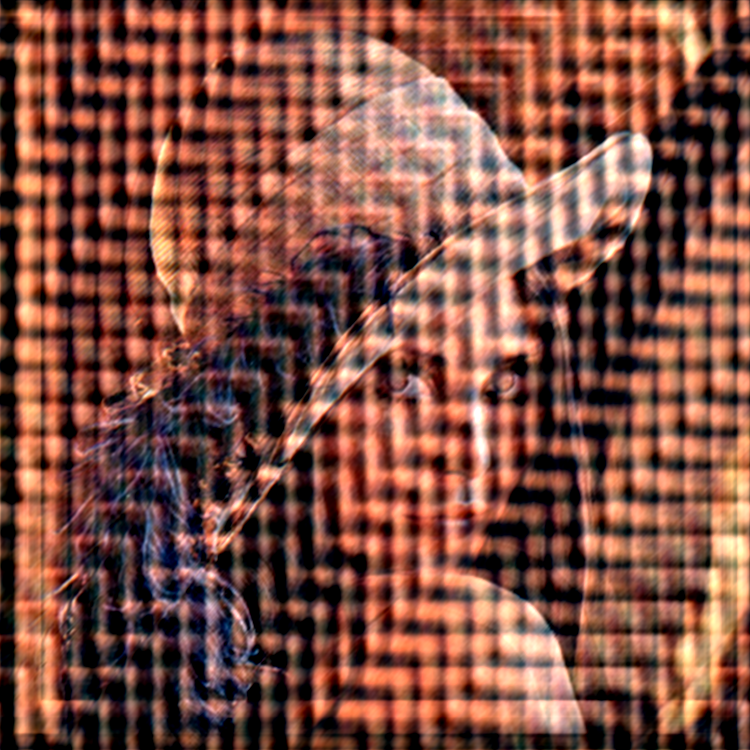
\includegraphics[{width= \textwidth}]{../Images/Results/Lena/Lena2/Reg-Comp.png}
\vspace{-30pt}
\caption{Picture deblurred using the whole image.}
\label{fig:Regcom}
\end{subfigure}
\caption{Different matrix's size for the PSF estimation.}
\end{figure}

We see that in this case the compression significantly reduces the computation time with little visible differences between the deblurred image with compression or not (more artefacts with reguralisation). Deblurring with the Wiener is inconclusive here, this observation will be discussed in section of the color influence (????).

However, in some cases the length of blur can be estimated with less well with compression which may alter the results (particularly with the algorithm of Reguralisation that is realy sensitive to this parameter).

\subsection{Computation time of methods used}

By analyzing the table of the previous point that summerize the execution time whith compression, we can clearly establish an order of speed. Wiener method is very fast (around a second for an image with compression), then comes Regularization (about 3 [s]) and finally Lucy Richardson takes much longer (around 7 [s]).

%TODO Y a moyen de faire une petite anaylse de la complexité temporelle vous pensez ? 


\subsection{parameter of the length estimator}

%TODO Arnaud comme on avait parlé hier et l'influence du paramètre (disons P) qui vaut 3, 5 ou 8. Moi je comprend pas trop donc ca serait pas mal si on arrive à expliquer ça avec le graphique des pics et tout. ..\Images\Results\plaque\55 y a une la plaque floutée artificiellement à 55 pixels (et angle 0) et quand on prend que P = 3 ou 5 (1 ou 2 dans le GUI), ça estime la longueur à 23 (à la place de 55), du coup ça donne Lucy_P1 Wiener_P1 et Reg_P1 (de la merde...). Tandis que P = 8 (3 dans le GUI) estime la longueur à 54, et ça donne les beaux résultats Lucy_P3 Wiener_P3 et Reg_P3. Tu sais en tirer quelque chose ? 

\subsection{Colors influence}

First of all, there is an influence on the run time. Indeed, as already seen ([MATH section]), color images are stored in 3-dimensions matrix $M$ x $N$ x $3$. So they take longer to be processed that the same gray-scaled image, stored in a matrix $M$ x $N$.
Below are the results obtained with the algorithm Lucy-Ridchrdson (with compression) for the photo of Lena and they gray-scaled one corresponding, both artificially blurred with an angle of 50 degrees and a length of 80 pixels:

% EN fait la longueur de floutage à été fixée à la bonne valeur pour la NB parce qu'ou sinon ca estime super mal, il faudrait voir pourquoi... Mais on est pas obligés de le dire dans le rapport :p 

%TODO mettre en images [Blur80a50 Lucy; Blur80a50NB LucyNB] temps d'execution color : 6,98[s], NB : 2,41[s]
 
%TODO voir pourquoi Wiener beug parfois selon les couleurs

\subsection{reals images}

%TODO mettre les images ..\Images\Results\reel\foot [Original L; W Reg]. et aussi ..\Images\Results\reel\mur [Original L; W R]
 
The results are pretty conclusive so far as the original blurred follows a minimum the assumptions which is not always given. Generally, Reguralisation is not valid for real images, this is explained by the fact that this method is very sensitive to the length parameter estimation and noise. However, in an image with a real blur, it's more difficult to properly estimate the length (blur not linear, "speed" of blurring non-constant) and the noise is very present (including photos taken above by a amateur camera). Lucy and Wiener are stronger, making it more interesting algorithm. However, Lucy is better than Wiener, but in return the execution time is more important.

\subsection{conclusion}

The three methods each have their advantages and disadvantages. Reguralization method is fast but too sensitive to noise and estimation of length, it's so not very robust but still interesting from a theoretical perspective. By contrast, The other two methods are robust. Wiener has the advantage of being faster than Lucy but the results are generally worse than those of Lucy.
